%\RequirePackage{snapshot}
\documentclass[a4paper,KOMA,landscape]{powersem}
\usepackage[display,stmo]{ifmslide}
\usepackage{soul}
%\usepackage[dvips]{graphicx}
%% user definitions
\newcommand{\ifmslide}{{\code{ifmslide.sty}}}
\newcommand{\tp}{{\code{texpower{}} \cite{texpower} }}
\newcommand{\hf}{{\code{hyperref{}} \cite{hyperref} }}
\hypersetup{pdfauthor={Henrik Frisk and Stefan �stersj�}}
\hypersetup{pdftitle={Negotiating the Musical Work. \\An empirical study on the
inter-relation between composition, interpretation and performance.}}
\hypersetup{pdfsubject={presentation}}

\IfFileExists{cmtt.sty}{\usepackage[override]{cmtt}%
                        \newcommand{\bs}{{\mtt\\}}}{%
                        \newcommand{\bs}{{$\setminus$}}}%

\panelposition{bottom}
\panellogo{Ulomacvnege}
\releaselogo
\freelogo(190,135)[5cm]

%%%%%%%%%%%%%%%%%%%%%%%%%%%%%%%%%%%%%%%%%%%%%%%%%%%%%%%%%%%%%%%%%%%%
%\usepackage{thumbpdf}
%%%%%%%%%%%%%%%%%%%%%%%%%%%%%%%%%%%%%%%%%%%%%%%%%%%%%%%%%%%%%%%%%%%%
\begin{document}
\headskip=12mm
\sffamily

\orgname{Malm\"{o} Academy of Music - Lund University}

\title{\begin{minipage}[t]{0.98\textwidth}\begin{center}
      {\mdseries Negotiating the Musical Work. \\An empirical study on the
inter-relation between composition, interpretation and performance.}
    \end{center}\end{minipage}}

\author{\scalebox{1}[1.3]{Henrik Frisk \& Stefan \"{O}stersj\"{o}}}

\address{\href{mailto:henrik.frisk@mhm.lu.se}
  {henrik.frisk@mhm.lu.se} \href{mailto:stefan\_ostersjo@hotmail.com}{stefan\_ostersjo@hotmail.com}}
\orgurl{http://www.henrikfrisk.com}
\slidepagestyle{panel}
%%%%%%%%%%%%%%%%%%%%%%%%%%%%%%%%%%%%%%%%%%%%%%%%%%%%%%%%%%%%%%%%%%%%
\begin{slide}
 \maketitle
\end{slide}
%%%%%%%%%%%%%%%%%%%%%%%%%%%%%%%%%%%%%%%%%%%%%%%%%%%%%%%%%%%%%%%%%%%%
\begin{slide}
  \section{Overview}
  \pause
  \liststepwise
      {
        \begin{itemize}
	 \item{Pre-study for a new work for guitar and computer - }
	 \step{\item{a study of the inter-relations between composer and performer.}}
	 \step{\item{Using a semiotic method of analysis drawing on Jean Molino and
	      Jean-Jacques Nattiez.}}
	 \step{\item{Analysis of fragments of a work for Harp and computer.}}
	 \step{\item{Analysis of a video recording of a
	      composer/performer session.}}
	 \step{\item{Discussion and conclusion(s).}}
         \end{itemize}
      }
\end{slide}
%%%%%%%%%%%%%%%%%%%%%%%%%%%%%%%%%%%%%%%%%%%%%%%%%%%%%%%%%%%%%%%%%%%%

%%%%%%%%%%%%%%%%%%%%%%%%%%%%%%%%%%%%%%%%%%%%%%%%%%%%%%%%%%%%%%%%%%%%
\begin{slide}
  \section{Introduction}
  \subsection{Conditions and purpose}
  \pause
  \liststepwise
      {
        \begin{itemize}
	 \item{The musical work before its ultimate notation and performance}
	 \step{\item{Mixed media music}}
	 \step{\item{Wish to gain a deeper understanding for the
	      underlying processes in the communication between the
	      composer and the performer.}}
	 \step{\item{Making use of this knowledge when designing artificial interactive systems.}}
        \end{itemize}
      }
\end{slide}
%%%%%%%%%%%%%%%%%%%%%%%%%%%%%%%%%%%%%%%%%%%%%%%%%%%%%%%%%%%%%%%%%%%%

%%%%%%%%%%%%%%%%%%%%%%%%%%%%%%%%%%%%%%%%%%%%%%%%%%%%%%%%%%%%%%%%%%%%
\begin{slide}
 \section{Construction/reproduction}
      \liststepwise
      {
      \step{Traditional view}

      \step
            {
              \begin{minipage}[h]{\textwidth}\begin{center}
                  {\includegraphics[width=0.9\textwidth]{img/cons-rep.pdf}} \end{center}
              \end{minipage}
            }

	    \step{Our experience of a more non-static inter-relation.}

	    \step 
	    {
              \begin{minipage}[h]{\textwidth}\begin{center}
                  {\includegraphics[width=0.9\textwidth]{img/cons-rep-rep-cons.pdf}} \end{center}
              \end{minipage}
            }
      }
\end{slide}
%%%%%%%%%%%%%%%%%%%%%%%%%%%%%%%%%%%%%%%%%%%%%%%%%%%%%%%%%%%%%%%%%%%%

%%%%%%%%%%%%%%%%%%%%%%%%%%%%%%%%%%%%%%%%%%%%%%%%%%%%%%%%%%%%%%%%%%%%
\begin{slide}
  \section{Music and notation}
  \liststepwise
      {
	 \step{Trevor Wishart: notation creates the crucial priorities
	      in the system - } \step{pitch and duration. \cite{wis96}}

	 \step{The split of 'the musician' into two agents.}

	 \step{What does the composer and the performer provide to the creative process?}
      }
\end{slide}
%%%%%%%%%%%%%%%%%%%%%%%%%%%%%%%%%%%%%%%%%%%%%%%%%%%%%%%%%%%%%%%%%%%%

%%%%%%%%%%%%%%%%%%%%%%%%%%%%%%%%%%%%%%%%%%%%%%%%%%%%%%%%%%%%%%%%%%%%
\begin{slide}
  \section{The two agents}
  \liststepwise
      {
      \step{Dialectic interplay between creation and interpretation.}

      \step{``Performances are necessarily constructive; that is, they
      necessarily add features that the work leaves vague or
      undetermined.''\cite{stecker} }

      \step{Authenticity in mixed media works.}

      \step{Programming of computer part - a special case of notation.}
      \step{How is this kind of notation transcribed and communicated to
      the performer?}

      \step{Different forms of authenticity: a creative field of tension in
      which the composer and the performer negotiate towards a version
      of the work.}
      }
\end{slide}
%%%%%%%%%%%%%%%%%%%%%%%%%%%%%%%%%%%%%%%%%%%%%%%%%%%%%%%%%%%%%%%%%%%%

%%%%%%%%%%%%%%%%%%%%%%%%%%%%%%%%%%%%%%%%%%%%%%%%%%%%%%%%%%%%%%%%%%%%
\begin{slide}
  \section{Semiology}
  \liststepwise
      {
	 \step{The nature of musical signification. \cite{nat89}}

	 \step{Nicolas Ruwet: Music - a language that signifies itself.}

	 \step{Jean Molino: ``On the one hand, the
	 unchallengeable presence of evocation; on the other, the impossibility
	 of exploiting it.'' \cite{molino}}

	 \step{Umberto Eco: ``Any attempt to establish
	 the referrent of a sign will force us to define this referrent with the
	 terminology of an abstract entity.'' \cite{eco71}}

	 \step{The composer/performer interaction creates a subculture -
      	 a cultural context in relation to which a semiologic analysis can
      	 be performed.}
      }
\end{slide}
%%%%%%%%%%%%%%%%%%%%%%%%%%%%%%%%%%%%%%%%%%%%%%%%%%%%%%%%%%%%%%%%%%%%

%%%%%%%%%%%%%%%%%%%%%%%%%%%%%%%%%%%%%%%%%%%%%%%%%%%%%%%%%%%%%%%%%%%%
\begin{slide}
  \section{The three dimensions}
  \liststepwise { 

  \step{Molino: the notion of a 'single, well-defined item of information
      to be transmitted, all the rest being simply noise' is
      'dangerously inaccurate and misleading as soon as we move from the
      artificial communication of information to a concrete act of human
      communication as a total social fact.'}  
      
      \step{Duchamp: two poles, the artist and the viewer. The intention of
      the artist holds no significance to the viewer.}

      \step{Val\'{e}ry: 'there is no guarantee of a direct
      correspondance between the effect produced by a work of art and the
      intentions of its creator'.} 

      \step{A model of analysis on three levels:}
          \step
              {
                \begin{itemize}
                \item{the poietic - the constructive phase}
                  \step{\item{the esthesic - the interpretative phase}}
                  \step{\item{the neutral - the trace}}
                \end{itemize}
              }
}
\end{slide}
%%%%%%%%%%%%%%%%%%%%%%%%%%%%%%%%%%%%%%%%%%%%%%%%%%%%%%%%%%%%%%%%%%%%

%%%%%%%%%%%%%%%%%%%%%%%%%%%%%%%%%%%%%%%%%%%%%%%%%%%%%%%%%%%%%%%%%%%%
\begin{slide}
  \section{Empirical studies}
  \subsection{Harp piece}
  \liststepwise
      {
      \step
            {
              \begin{minipage}[h]{\textwidth}\begin{center}
                  {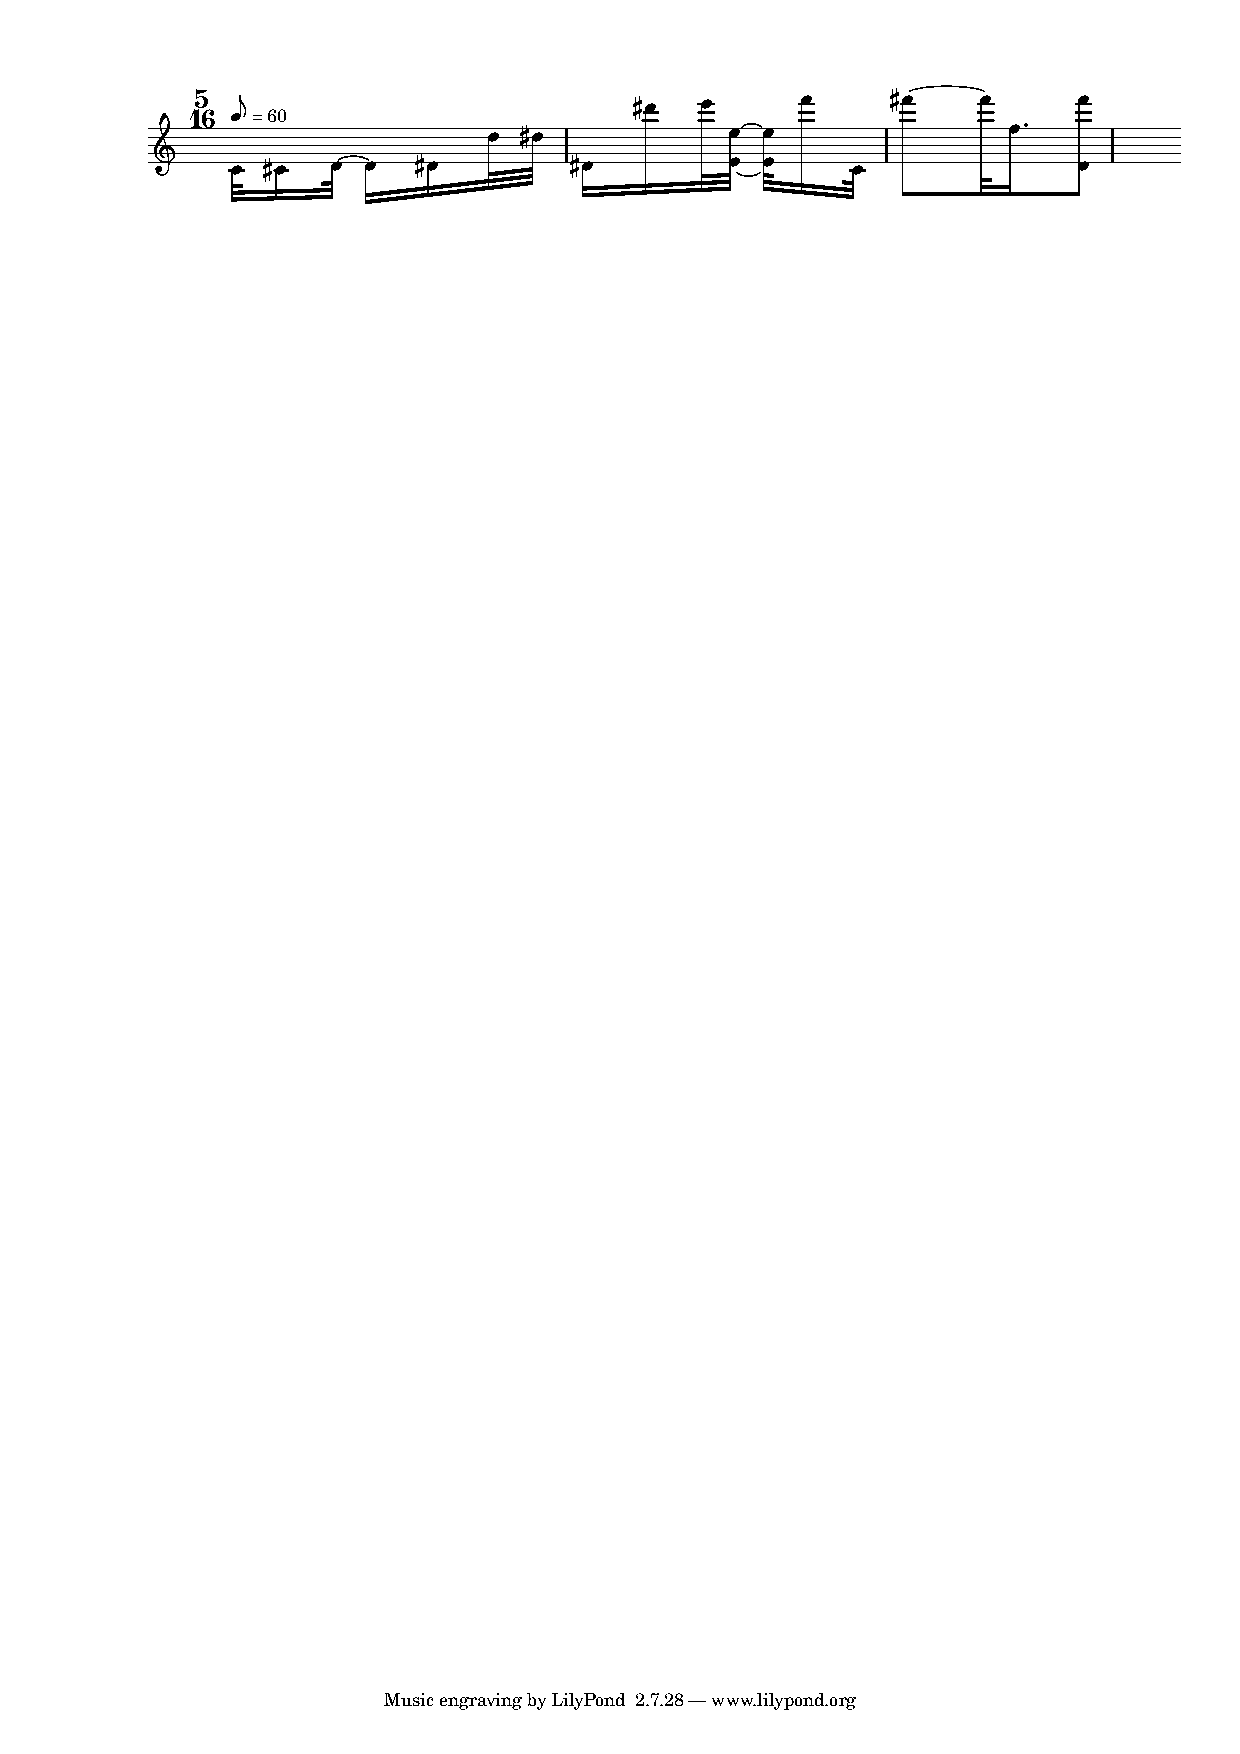
\includegraphics[width=0.9\textwidth]{img/score/eps/harpVersion1}} \end{center}
              \end{minipage}
            }
      \step
            {
              \begin{minipage}[h]{\textwidth}\begin{center}
                  {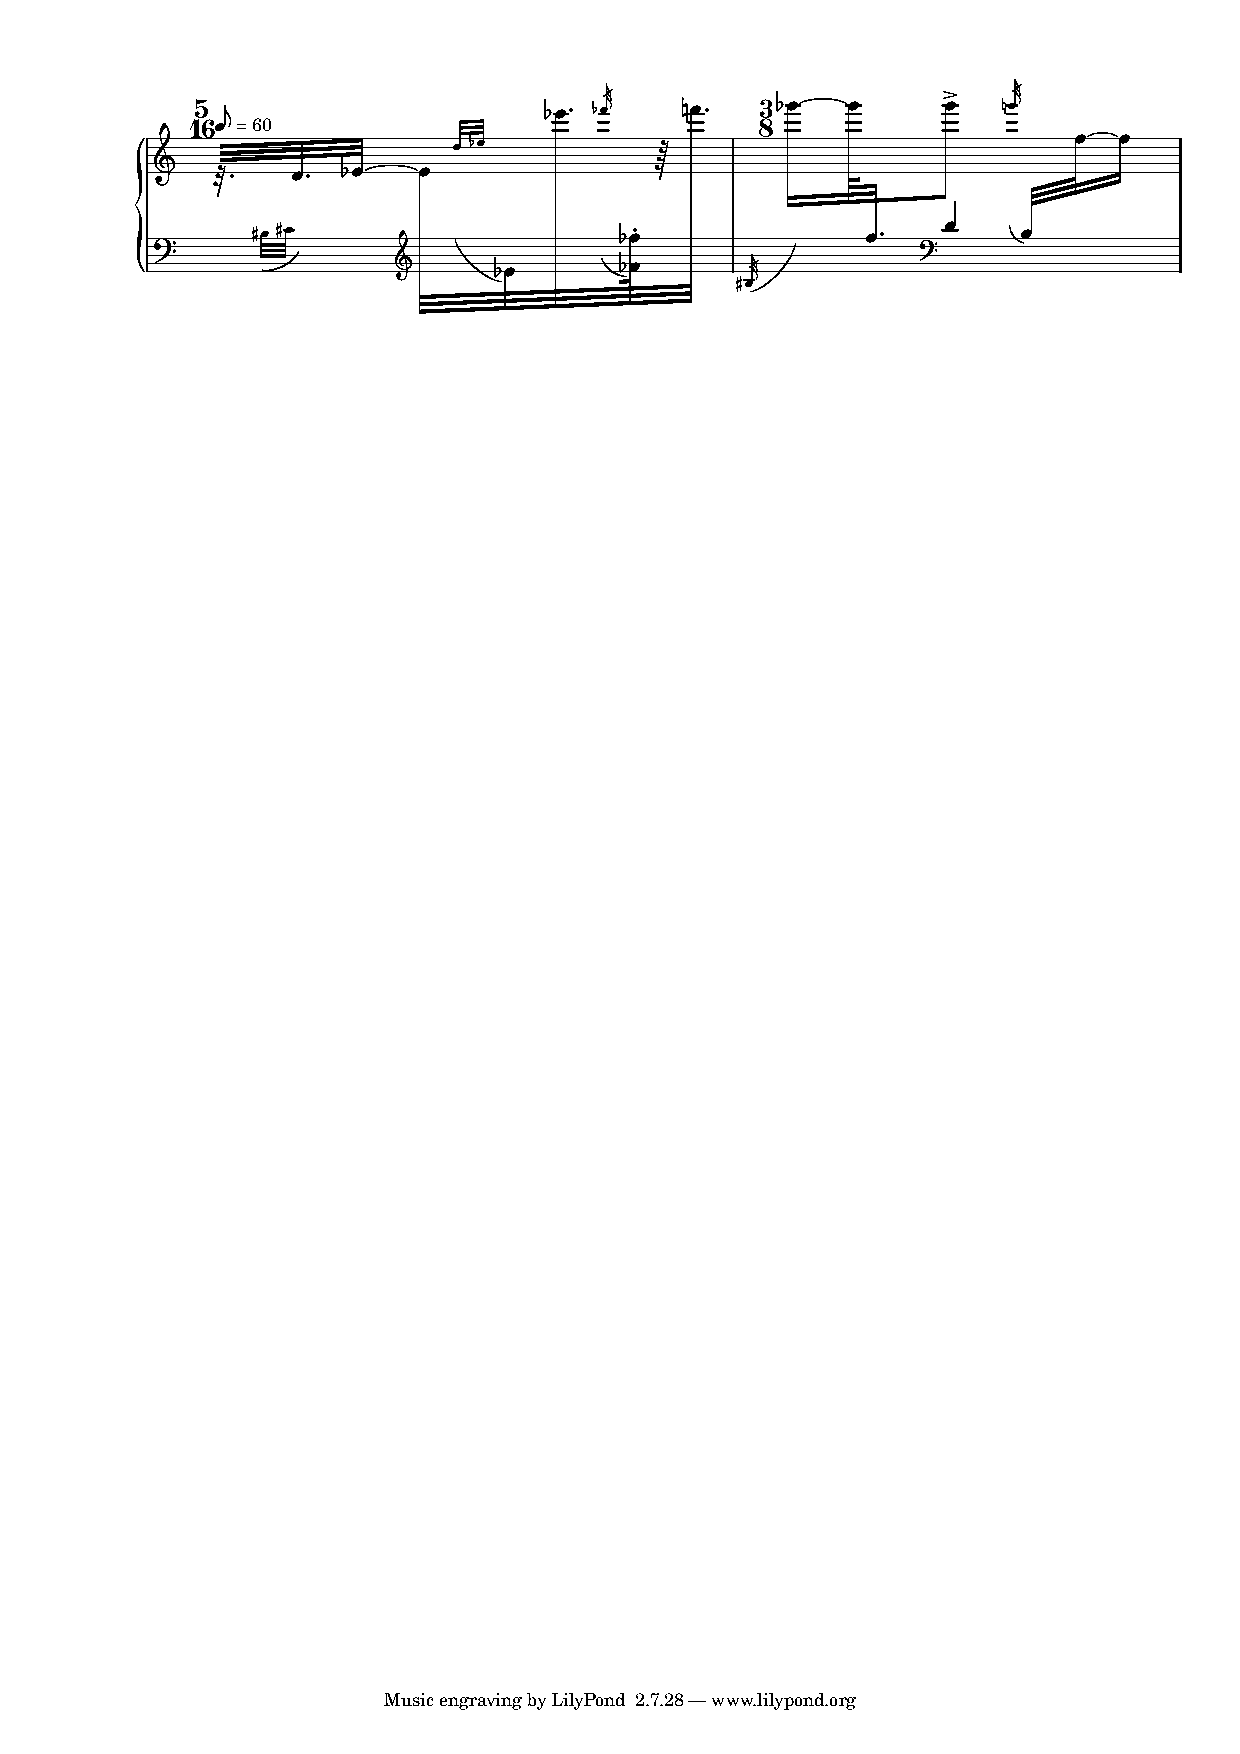
\includegraphics[width=0.9\textwidth]{img/score/eps/harpVersion2}} \end{center}
              \end{minipage}
            }
      }
\end{slide}
%%%%%%%%%%%%%%%%%%%%%%%%%%%%%%%%%%%%%%%%%%%%%%%%%%%%%%%%%%%%%%%%%%%%

%%%%%%%%%%%%%%%%%%%%%%%%%%%%%%%%%%%%%%%%%%%%%%%%%%%%%%%%%%%%%%%%%%%%
\begin{slide}
  \section{Harp piece}
  \liststepwise
      {
      \step
            {
              \begin{minipage}[h]{\textwidth}\begin{center}
                  {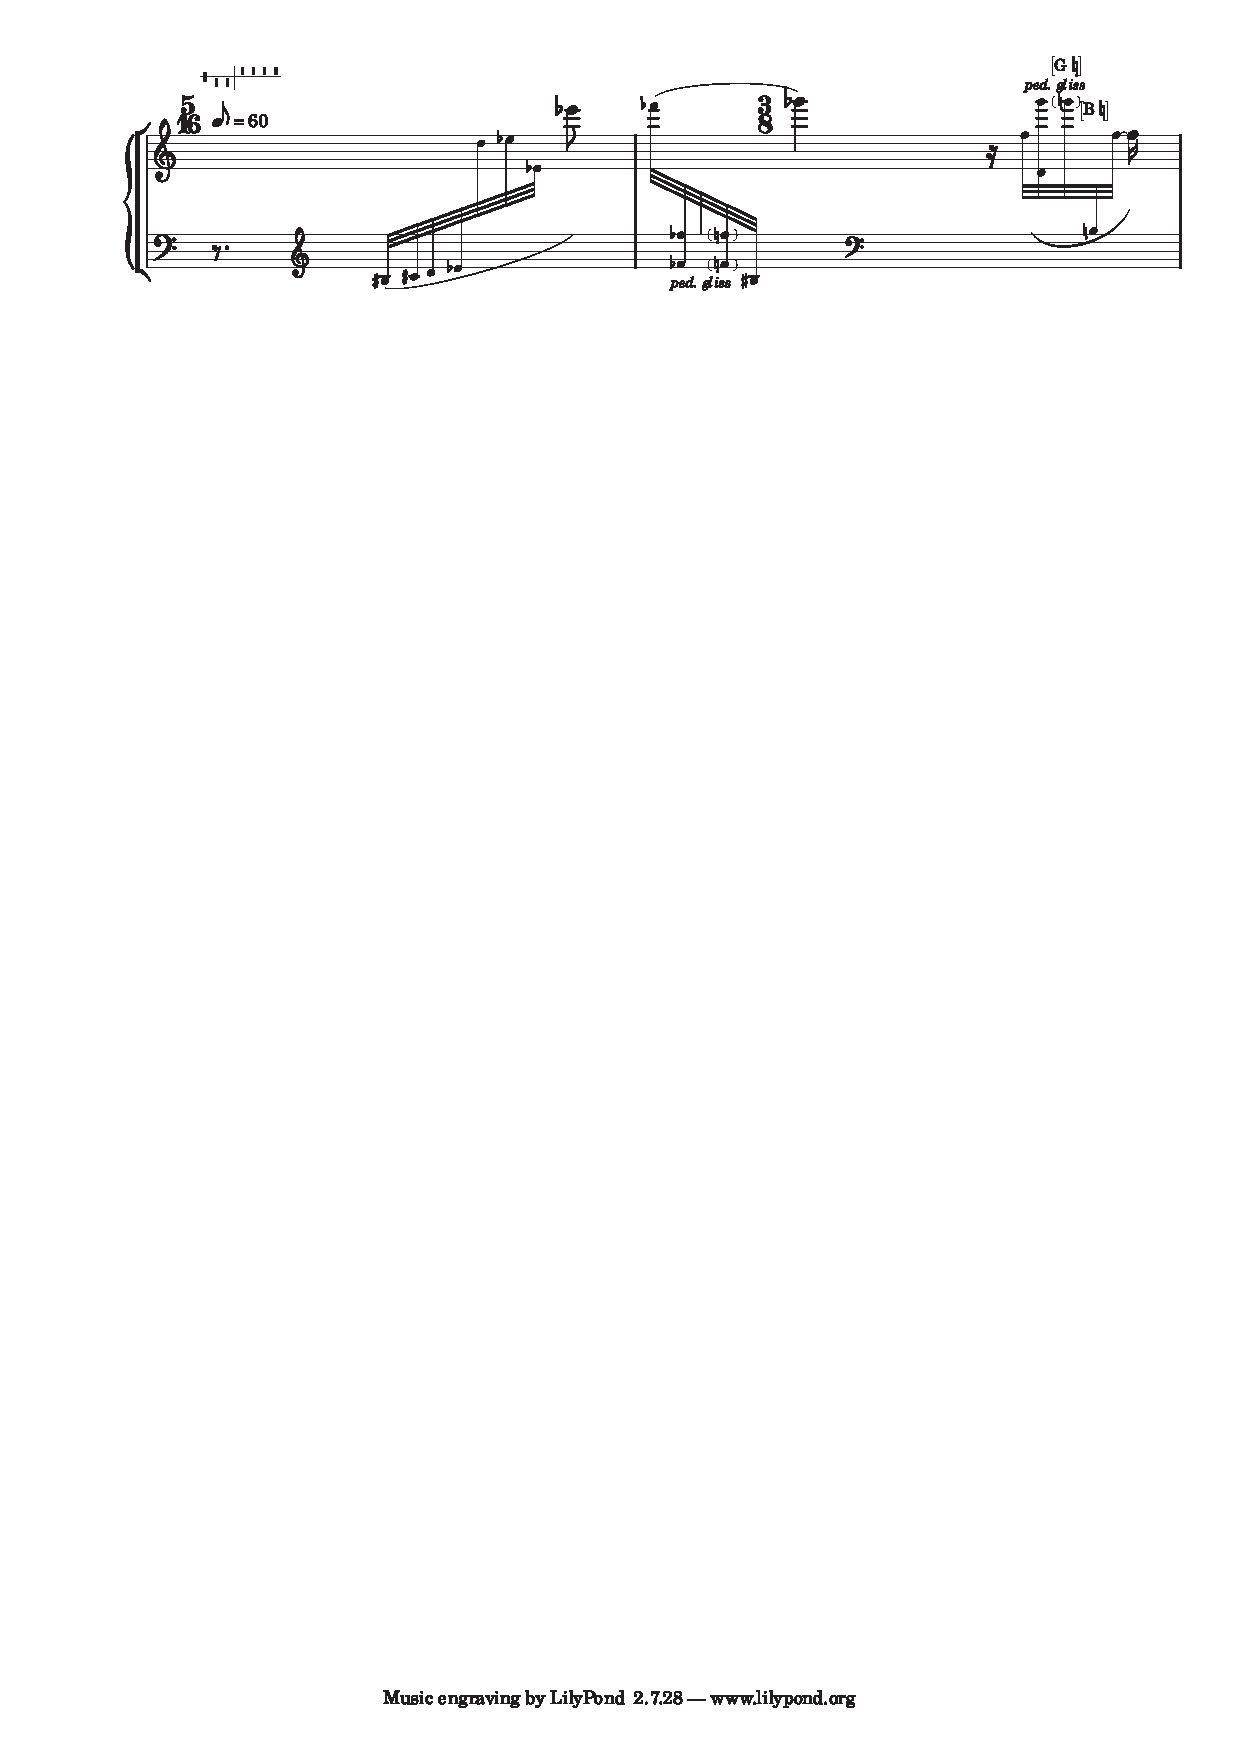
\includegraphics[width=0.9\textwidth]{img/score/eps/harpVersion3}} \end{center}
              \end{minipage}
            }
      \step
            {
              \begin{minipage}[h]{\textwidth}\begin{center}
                  {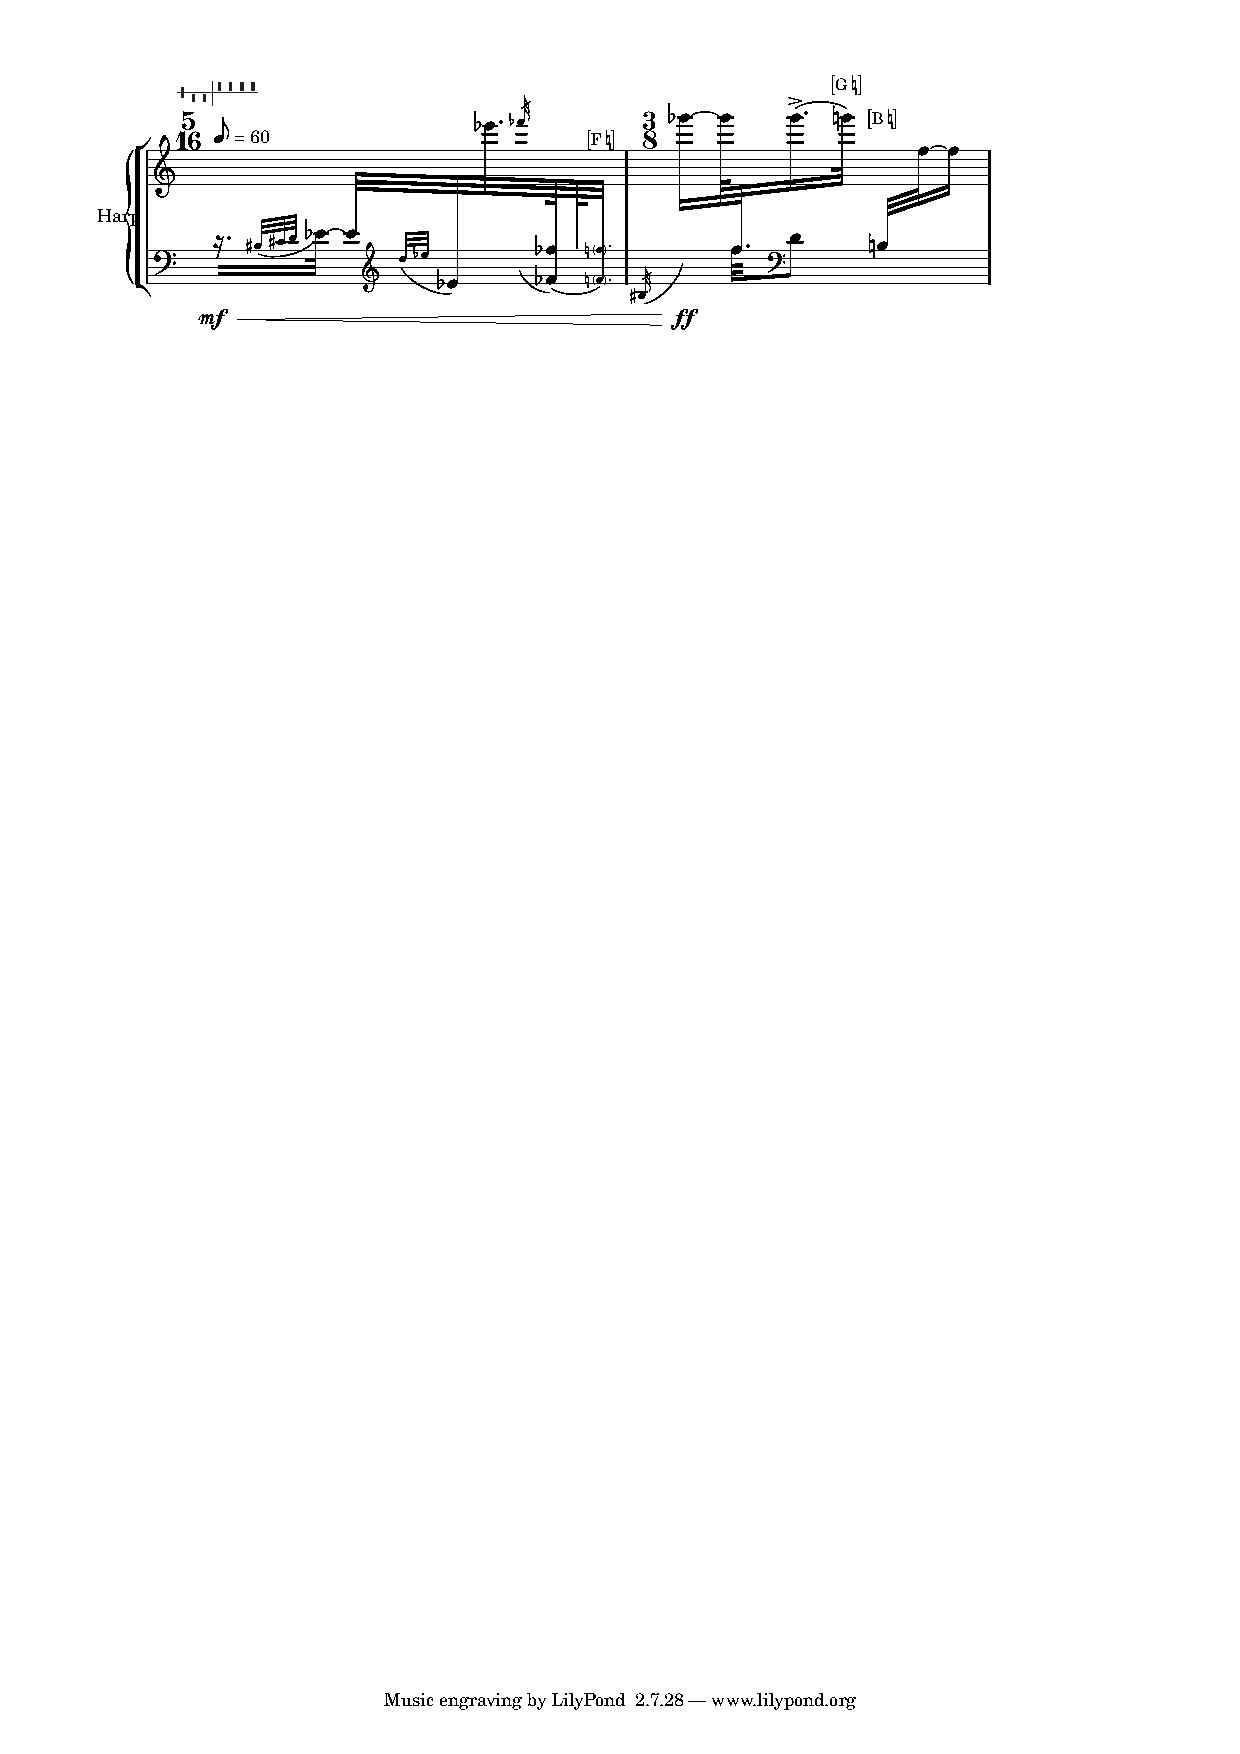
\includegraphics[width=0.9\textwidth]{img/score/eps/harpVersion4}} \end{center}
              \end{minipage}
            }
      }
\end{slide}
%%%%%%%%%%%%%%%%%%%%%%%%%%%%%%%%%%%%%%%%%%%%%%%%%%%%%%%%%%%%%%%%%%%%

%%%%%%%%%%%%%%%%%%%%%%%%%%%%%%%%%%%%%%%%%%%%%%%%%%%%%%%%%%%%%%%%%%%%j

\slidepagestyle{empty}
\begin{slide}
\bibliography{bibliography}
\bibliographystyle{apalike}
\end{slide}
%%%%%%%%%%%%%%%%%%%%%%%%%%%%%%%%%%%%%%%%%%%%%%%%%%%%%%%%%%%%%%%%%%%%
\end{document}
%%%%%%%%%%%%%%%%%%%%%%%%%%%%%%%%%%%%%%%%%%%%%%%%%%%%%%%%%%%%%%%%%%%%
%%%%%%%%%%%%%%%%%%%%%%%%%%%%%%%%%%%%%%%%%%%%%%%%%%%%%%%%%%%%%%%%%%%%


